\chapter{Pendahuluan}
\pagenumbering{arabic}

\section{Latar Belakang}

Pengendalian termal satelit bertujuan untuk menjaga semua komponen satelit
tetap pada rentang suhu operasional pada selama masa misi satelit. Desain
sistem kendali termal yang buruk dapat mengakibatkan kerusakan permanen pada
komponen satelit akibat panas berlebih atau kondisi non-operasional yang fatal
dalam misi akibat suhu komponen yang terlalu rendah. Semakin dekat model termal
satelit dengan karakteristik termal satelit yang sebenarnya, semakin kecil pula
kemungkinan suhu satelit mencapai nilai di luar rentang yang sudah ditentukan.
Karena itu, desain sistem kendali termal satelit yang baik membutuhkan
pemodelan termal satelit yang baik pula. Hal ini membuat proses desain sistem
kendali termal satelit menjadi salah satu tahap yang paling penting dalam
periode pengembangan satelit.

Permasalahan yang mungkin dihadapi pada proses desain sistem termal satelit
antara lain muncul karena karakteristik termal satelit ditentukan oleh banyak
parameter yang saling bergantung sama lain. Untuk memodelkan karakteristik
termal satelit secara akurat, tentunya dibutuhkan perhitungan parameter satelit
yang akurat juga. Selain itu, desain sistem kendali termal satelit harus turut
memperhitungkan batasan satelit lain seperti ruang, daya, dan berat.

Pada kasus satelit mikro dan nano, ukuran satelit yang kecil dapat berakibat
pada kapasitas termal yang kecil pula sehingga satelit mudah mengalami
perubahan suhu. Satelit mikro dan nano juga biasanya hanya bergantung pada
sistem kendali termal pasif akibat batasan ketersediaan daya. Akibatnya,
seringkali diperlukan langkah tambahan pada saat operasi untuk memastikan
satelit dapat tetap dijaga pada rentang suhu operasional. 

Permasalahan di atas terjadi pada LAPAN-A3, satelit yang memiliki misi utama
observasi Bumi serta diluncurkan pada tahun 2016. LAPAN-A3 merupakan satelit
yang dikembangkan Lembaga Penerbangan dan Antariksa Nasional (LAPAN) dengan
kerja sama dengan Institut Pertanian Bogor (IPB) setelah sebelumnya LAPAN telah
berhasil meluncurkan satelit LAPAN-A1 dan LAPAN-A2. Ketiga satelit tesebut
termasuk dalam kategori mikrosatelit serta menggunakan sistem kendali termal
pasif dengan cara distribusi panas lewat struktur dan penggunaan cat khusus
untuk memantulkan radiasi. Akan tetapi, berbeda dengan LAPAN-A1 dan LAPAN-A2,
LAPAN-A3 membutuhkan maneuver khusus untuk menjaga suhu \textit{payload}
utamanya tetap pada rentang suhu operasional.

LAPAN-A3 memiliki \textit{payload} utama berupa pencitra multispektral yang
harus dijaga pada rentang suhu operasional 0 sampai dengan 70 \degree C. Dari
hasil observasi data telemetri, ditemukan bahwa suhu pencitra turun hingga
mencapai nilai negatif pada periode bulan Mei sampai dengan Juni
\cite{ribah2019}. Kondisi ini berakibat buruk pada operasi satelit LAPAN-A3
karena pencitra tidak dapat dioperasikan pada suhu di bawah 0 \degree C
sehingga frekuensi misi pengambilan citra berkurang. Observasi lebih lanjut
menemukan hubungan fenomena penurunan suhu pencitra dengan variasi sudut
\textit{beta} orbit satelit akibat perubahan musim. Untuk menaikkan suhu
pencitra dan melawan penurunan sudut \textit{beta} orbit, operator LAPAN-A3
harus memberikan perintah maneuver \textit{stop and release} serta \textit{stop
and release with roll} sehingga sisi satelit yang memuat pencitra menerima
paparan sinar Matahari lebih banyak.

Dapat dilihat bahwa perlindungan termal pasif pada struktur LAPAN-A3 berupa
alumunium yang telah diberi anode hitam sendiri saja tidak dapat memenuhi
persyaratan termal LAPAN-A3. Selain itu, penggunaan maneuver khusus tetap
memiliki konsekuensi negatif terhadap operasi harian LAPAN-A3. Pertama,
pencitra harus dimatikan selama durasi maneuver. Hal ini tetap berakibat pada
berkurangnya frekuensi misi pengambilan citra. Kemudian, maneuver khusus
membuat satelit terkunci dalam sikap \textit{off-nadir pointing} selama durasi
maneuver. Akibatnya, misi yang membutuhkan sikap \textit{nadir pointing} tidak
bisa dilakukan dan harus dikompensasi dengan misi lain yang tidak membutuhkan
\textit{nadir pointing} seperti pengukuran medan magnet Bumi. Karena itu, jelas
dibutuhkan sebuat model termal satelit sederhana baru yang dapat digunakan
sebagai referensi dalam pengembangan satelit-satelit LAPAN selanjutnya agar
permasalahan yang ada saat ini tidak terjadi lagi.

Analisis termal satelit konvensional dilakukan dengan menyelesaikan persamaan
termal satelit yang sudah dimodelkan menjadi beberapa titik analisis atau node
lewat perhitungan numerik atau simulasi perangkat lunak komersial. Untuk
satelit dalam kelas mikro, Das et al. \cite{das} telah mengembangkan prosedur
desain termal satelit sederhana menggunakan pendekatan pertama lewat
penyelesain persamaan termal satelit multi-nodal yang disederhanakan. Kemudian,
pendekatan kedua sudah dilakukan oleh Boudjemai et al. \cite{boudjemai2015}
yang menggunakan metode elemen hingga untuk menganalisis karakteristik termal
baterai satelit.

Karena LAPAN belum memiliki perangkat lunak yang dibutuhkan
\cite{budiantoro2019}, metode yang mungkin dipakai hanya metode perhitungan
numerik. Pendekatan ini membutuhkan perhitungan banyak parameter satelit secara
akurat bahkan untuk model satelit 1 node sekalipun. Akibatnya, penggunaan
metode perhitungan numerik biasanya terbatas untuk model satelit 1, 2, atau 3
node saja. Untuk model multi-nodal, pendekatan yang umum digunakan adalah
metode kedua berupa simulasi lewat perangkat lunak komersial. Sebagai contoh,
Totani et al. \cite{totani2014} menjelaskan prosedur desain termal satelit
kelas mikro dan nano menggunakan metode perhitungan numerik untuk pendekatan
satelit 1 dan 2 node saja. Pada karya tulis yang sama, prosedur desain termal
satelit dengan pendekatan multi-nodal dilakukan dengan bantuan perangkat lunak
SINDA/FLUINT. Selain itu, sampai karya tulis ini dibuat, ketiga karya tulis
yang telah disebutkan belum memberikan validasi metode yang diajukan dengan
data operasi aktual satelit.

Berdasarkan alasan yang telah dijelaskan di atas, penelitian pada karya tulis
ini bertujuan untuk menjabarkan langkah-langkah pembuatan model termal satelit
sederhana yang dapat mengurangi jumlah parameter satelit yang harus dihitung
serta dapat divalidasi dengan data telemetri satelit. Prosedur pembuatan model
termal tersebut akan diimplementasikan pada satelit LAPAN-A3. Diharapkan bahwa
model termal yang dihasilkan pada karya tulis ini dapat memprediksi suhu
satelit secara akurat sehingga satelit LAPAN di masa depan dapat memiliki
prediksi suhu komponen yang lebih akurat juga. Model termal yang lebih akurat
juga akan memungkinkan lebih banyak misi pencitraan multispektral seperti dalam
LAPAN-A4 atau \textit{payload} yang mengeluarkan panas seperti
\textit{Synthetic Apperture Radar} (SAR) pada LAPAN-A5/Chibasat.


Pada karya tulis ini, metode Machine Learning akan digunakan untuk membuat
model termal semi-empiris berbasis data telemetri satelit aktual serta
perhitungan faktor lingkungan serta orbit satelit. Penggunaan metode Machine
Learning bukanlah fenomena baru dalam analisis termal satelit. Sebagai contoh,
metode Machine Learning telah digunakan untuk membuat simulasi termal satelit
\textit{real-time} \cite{junior2017}, mempermudah iterasi dalam proses desain
sistem kendali termal satelit \cite{escobar2016}, serta mengoptimasi desain termal satelit
\cite{xiong2020}.

Dengan demikian, diharapkan hasil akhir dari karya tulis ini adalah prosedur
pemodelan termal semi-empiris satelit LAPAN-A3 menggunakan metode Machine
Learning yang dapat memprediksi suhu ke-7 node satelit (6 node untuk setiap
sisi satelit dan 1 node untuk plat tengah satelit) selama periode observasi 19
sampai dengan 20 Mei 2018. Penggunakan metode Machine Learning dilakukan untuk
mengurangi jumlah variabel yang harus dihitung untuk memodelkan karakteristik
termal satelit secara akurat. Hasil prediksi suhu dari model termal satelit
juga akan dievaluasi untuk memvalidasi keakuratan model termal serta mengukur
potensi model di masa depan.

\section{Rumusan Masalah}

Dari latar belakang yang telah dijelaskan sebelumnya, dapat dibuat rumusan masalah sebagai berikut :

\begin{enumerate}
\item Bagaimana pemodelan termal semi-empiris satelit LAPAN-A3 menggunakan metode Machine Learning dapat dilakukan?
\item Bagaimana perbandingan perubahan suhu sisi-sisi satelit hasil prediksi model termal satelit dengan data telemetri satelit?
\item Bagaimana performa model termal satelit yang dihasilkan?
\end{enumerate}

\section{Tujuan Penelitian}

Berlandaskan rumusan masalah, penelitian pada karya tulis ini bertujuan untuk :

\begin{enumerate}
\item Melakukan penjabaran langkah-langkah untuk membuat model termal satelit multi-nodal secara semi-empiris menggunakan metode Machine Learning
\item Membuat model termal satelit yang dapat memprediksi perubahan suhu sisi-sisi satelit LAPAN A3
\item Membandingkan perubahan suhu node satelit hasil prediksi model termal dengan data telemetri satelit
\item Menganalisis performa hasil prediksi dari model termal satelit yang telah dibuat
\end{enumerate}

\section{Batasan Penelitian}

Penelitian dalam karya tulis ini dibatasi sebagai berikut :

\begin{enumerate}
\item Pemodelan termal satelit LAPAN A3 dilakukan untuk periode observasi 19-20 Mei 2018
\item Selama periode observasi, satelit dianggap tidak mengalami perubahan massa dan karakteristik termal
\item Satelit LAPAN A3 dianggap berbentuk balok dan dibagi menjadi 7 titik analisis atau node : 6 sisi satelit dan plat tengah satelit
\end{enumerate}

\section{Metodologi}

Gambar~\ref{fig:metodologi} memuat metodologi pembuatan karya tulis ini. Secara umum,
penelitian dimulai dengan studi pustaka topik terkait pemodelan termal satelit
dan metode Machine Learning. Selanjutnya, dilakukan pengumpulan data yang
dibutuhkan untuk pemodelan termal satelit. Kemudian, dilakukan pembuatan
dataset dalam format yang sesuai untuk digunakan dalam pembuatan model Machine
Learning. Lalu, dataset tersebut dibagi menjadi 2 set : set latihan untuk
membantu model regresi linear Machine Learning dalam mengidentifikasi fitur dan
tren perubahan suhu satelit dan set ujian untuk mendapatkan prediksi perubahan
suhu satelit dari model Machine Learning. Terakhir, hasil prediksi suhu satelit
dari model Machine Learning dievaluasi.

\begin{figure}[H]
\setlength\belowcaptionskip{-0.7\baselineskip}
\begin{center}
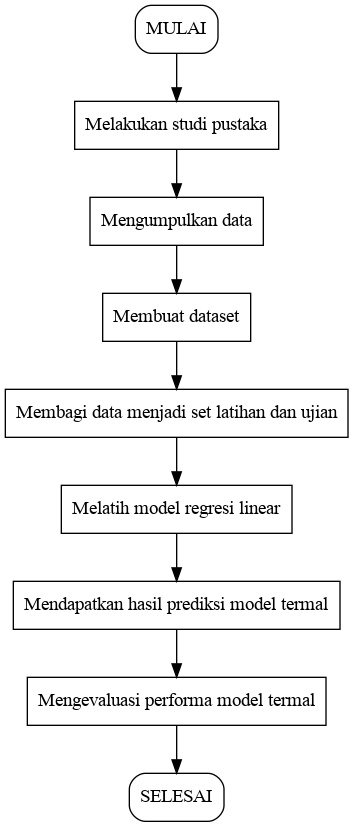
\includegraphics[width=0.4\textwidth]{fig/graph_metodologi.png}
\caption{Metodologi penelitian karya tulis}
\label{fig:metodologi}
\end{center}
\end{figure}

Proses pembuatan dataset untuk model termal satelit memiliki algoritma
tersendiri yang disajikan pada Gambar \ref{fig:algoritma}. Secara singkat,
pembuatan dataset model termal satelit terdiri dari 3 langkah utama : penyiapan
dataset dasar, perhitungan faktor-faktor panas satelit, dan penyaringan
dataset. Penjelasan lebih menyeluruh terkait proses pembuatan dataset akan
dibahas pada Bab Pemodelan Termal Satelit LAPAN-A3.

\begin{figure}[H]
\setlength\belowcaptionskip{-0.7\baselineskip}
\begin{center}
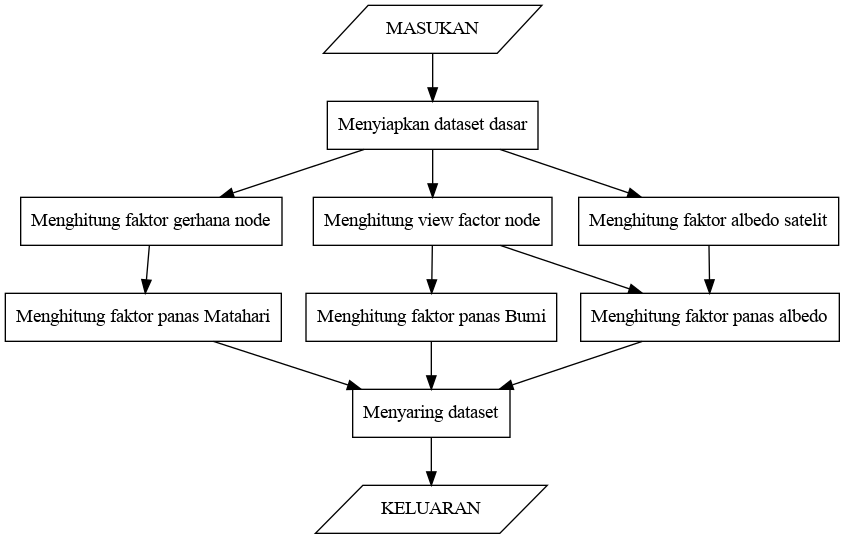
\includegraphics[width=0.75\textwidth]{fig/graph_algoritma.png}
\caption{Algoritma pembuatan dataset}
\label{fig:algoritma}
\end{center}
\end{figure}

\section{Sistematika Penulisan}

Sistematika penulisan karya tulis ini adalah sebagai berikut :

\begin{enumerate}
\item BAB I PENDAHULUAN

Bab ini membahas latar belakang, rumusan masalah, tujuan penelitian, batasan
penelitian, metodologi penelitian, dan sistematika penulisan.

\item BAB II TINJAUAN PUSTAKA

Bab ini membahas dasar teori yang digunakan dalam penelitian dalam rangka
pengerjaan karya tulis ini.

\item BAB III PEMODELAN TERMAL SATELIT LAPAN-A3

Bab ini menjabarkan langkah-langkah untuk membuat model termal semi-empiris
satelit LAPAN-A3 dengan menggunakan perangkat lunak Python.

\item BAB IV HASIL DAN ANALISIS

Bab ini berisi hasil prediksi suhu sisi-sisi satelit LAPAN-A3 serta analisis
kriteria korelasi dan performa model termal satelit LAPAN-A3 yang dihasilkan
dari bab sebelumnya.

\item BAB V KESIMPULAN DAN SARAN

Bab ini berisi kesimpulan dari penelitian yang telah dilakukan dan saran
untuk penelitian selanjutnya.
\end{enumerate}
